% ------------------------------------------------------------------------
% ------------------------------------------------------------------------
% abnTeX2: Modelo de Relatório Técnico/Acadêmico em conformidade com 
% ABNT NBR 10719:2015 Informação e documentação - Relatório técnico e/ou
% científico - Apresentação
% Versão mais enxuta para disciplina de Organização de Arquivos 2018
% ------------------------------------------------------------------------ 
% ------------------------------------------------------------------------

\documentclass[
	% -- opções da classe memoir --
	12pt,				% tamanho da fonte
	openany,			% capítulos começam em qualquer pagina
	twoside,			% para impressão em recto e verso. Oposto a oneside
	a4paper,			% tamanho do papel. 
	% -- opções da classe abntex2 --
	%chapter=TITLE,		% títulos de capítulos convertidos em letras maiúsculas
	%section=TITLE,		% títulos de seções convertidos em letras maiúsculas
	%subsection=TITLE,	% títulos de subseções convertidos em letras maiúsculas
	%subsubsection=TITLE,% títulos de subsubseções convertidos em letras maiúsculas
	% -- opções do pacote babel --
	english,			% idioma adicional para hifenização
	french,				% idioma adicional para hifenização
	spanish,			% idioma adicional para hifenização
	brazil,				% o último idioma é o principal do documento
	]{abntex2}


% ---
% PACOTES
% ---

% ---
% Pacotes fundamentais 
% ---
\usepackage{lmodern}			% Usa a fonte Latin Modern
\usepackage[T1]{fontenc}		% Selecao de codigos de fonte.
\usepackage[utf8]{inputenc}		% Codificacao do documento (conversão automática dos acentos)
\usepackage{indentfirst}		% Indenta o primeiro parágrafo de cada seção.
\usepackage{color}				% Controle das cores
\usepackage{graphicx}			% Inclusão de gráficos
\usepackage{microtype} 			% para melhorias de justificação
\usepackage{hyperref}
% ---

% ---
% Pacotes adicionais, usados no anexo do modelo de folha de identificação
% ---
\usepackage{multicol}
\usepackage{multirow}
% ---

% ---
% Pacotes de citações
% ---
\usepackage[brazilian,hyperpageref]{backref}	 % Paginas com as citações na bibl
\usepackage[alf]{abntex2cite}	% Citações padrão ABNT

% --- 
% CONFIGURAÇÕES DE PACOTES
% --- 

% ---
% Configurações do pacote backref
% Usado sem a opção hyperpageref de backref
\renewcommand{\backrefpagesname}{Citado na(s) página(s):~}
% Texto padrão antes do número das páginas
\renewcommand{\backref}{}
% Define os textos da citação
\renewcommand*{\backrefalt}[4]{
	\ifcase #1 %
		Nenhuma citação no texto.%
	\or
		Citado na página #2.%
	\else
		Citado #1 vezes nas páginas #2.%
	\fi}%
% ---

% ---
% Informações de dados para CAPA e FOLHA DE ROSTO
% ---
% colocar o título aqui (por exemplo, Documentação Externa Implementação B*-tree)
\titulo{Primeiro Trabalho Prático de Organização de Arquivos}
\autor{Fabio Fogarin Destro (10284667) \and Paulo A. de Oliveira Carneiro (10295304) \and Renata Vinhaga dos Anjos (10295263) \and Vítor H. Gratiere Torres (102849552)} %nomes dos integrantes do grupo aqui
\local{Universidade de São Paulo

Instituto de Ciências Matemáticas e Computação

Bacharelado em Ciências da Computação

Departamento de Ciências de Computação

SCC0215 - Organização de Arquivos

Professora Dra. Cristina Dutra de Aguiar Ciferri

9 de Maio de 2017, São Carlos, SP}
\data{}
\instituicao{%
  Universidade de São Paulo -- USP
  \par
  Instituto de Ciências Matemáticas e Computação -- ICMC
  \par
  Bacharelado em Ciências da Computação}
\tipotrabalho{Documentação Externa}
% O preambulo deve conter o objetivo, 
% o nome da instituição e a área de concentração 
\preambulo{Praticar conceitos aprendidos em aulas de Organização de Arquivos, na Universidade de São Paulo}
% ---

% ---
% Configurações de aparência do PDF final

% alterando o aspecto da cor azul
\definecolor{blue}{RGB}{41,5,195}

% informações do PDF
\makeatletter
\hypersetup{
     	%pagebackref=true,
		pdftitle={\@title}, 
		pdfauthor={\@author},
    	pdfsubject={\imprimirpreambulo},
	    pdfcreator={LaTeX with abnTeX2},
		pdfkeywords={abnt}{latex}{abntex}{abntex2}{relatório técnico}, 
		colorlinks=true,       		% false: boxed links; true: colored links
    	linkcolor=blue,          	% color of internal links
    	citecolor=blue,        		% color of links to bibliography
    	filecolor=magenta,      		% color of file links
		urlcolor=blue,
		bookmarksdepth=4
}
\makeatother
% --- 

% --- 
% Espaçamentos entre linhas e parágrafos 
% --- 

% O tamanho do parágrafo é dado por:
\setlength{\parindent}{1.3cm}

% Controle do espaçamento entre um parágrafo e outro:
\setlength{\parskip}{0.2cm}  % tente também \onelineskip

% Não utiliza capítulos, pois no nosso caso não vai ter utilização
\makeatletter
\renewcommand{\thesection}{%
  \ifnum\c@chapter<1 \@arabic\c@section
  \else \thechapter.\@arabic\c@section
  \fi
}
\makeatother

% ---
% compila o indice
% ---
\makeindex
% ---

% ----
% Início do documento
% ----
\begin{document}

% Seleciona o idioma do documento (conforme pacotes do babel)
%\selectlanguage{english}
\selectlanguage{brazil}

% Retira espaço extra obsoleto entre as frases.
\frenchspacing 

% ----------------------------------------------------------
% ELEMENTOS PRÉ-TEXTUAIS
% ----------------------------------------------------------
% \pretextual

% ---
% Capa
% ---
\imprimircapa
% ---

% ---
% Folha de rosto
% (o * indica que haverá a ficha bibliográfica)
% ---
%\imprimirfolhaderosto*
% ---

% ---
% inserir o sumario
% ---
\pdfbookmark[0]{\contentsname}{toc}
\tableofcontents*
\cleardoublepage
% ---


% ----------------------------------------------------------
% ELEMENTOS TEXTUAIS
% ----------------------------------------------------------
\textual

% ----------------------------------------------------------
% Introdução 
% ----------------------------------------------------------
\section{Introdução}

Este trabalho consiste na implementação de 9 funções que envolvem manipulação de dados. Dentre essas são: inserção, remoção e atualização de dados baseados na abordagem dinâmica de reaproveitamento de espaços de registros logicamente removidos.

O programa foi feito utilizando a linguagem \verb|C|, sendo compilado e testado no sistema operacional Linux (\verb|Ubuntu 16.04 lts|).

Pode-se garantir que o arquivo de dados ainda não exista antes da primeira execução: \verb|make clean|.

Para compilar: \verb|make all|.

Para executar o programa: \verb|./arquivo [FUNCAO] [...ARGUMENTOS...]|.

% ---
% Esta seção, utilizado por diferentes exemplos do abnTeX2, ilustra o uso de
% comandos do abnTeX2 e de LaTeX.
% ---

\section{Macros}
    Utilizamos algumas substituições de sintaxe para facilitar o entendimento e a generalização do código. Essas macros foram usadas no cálculo do \textit{Byte Offset}:
    \begin{itemize}
    \item \verb|TAM_CAMPO| - tamanho dos campos de tamanho fixo (10 bytes);
    \item \verb|TAM_TEG| - tamanho fixo para os registros do trabalho (112 bytes) como especificado;
    \item \verb|TAM_CABECALHO| - tamanho do cabeçalho do arquivo binário (5 bytes = 1 byte para status do arquivo + 4 bytes para o topo da pilha de remoção lógica).
    \end{itemize}

\section{Estrutura de Dados}
    Usamos duas \verb|structs| para auxílio e armazenamento temporário de dados para manipulação:
     \begin{itemize}
     \item  \verb|Cabeçalho|: contém  o status do arquivo \verb|saida.bin| (\verb|0| para inconsistente e \verb|1| para consistente) e o topo da pilha de registros logicamente removidos (\verb|-1| quando não há registros removidos);
    \item \verb|Escola|: contém o código da escola e cinco ponteiros para as datas de Início e Final do ano letivo escolar (de tamanho fixo),  para os nomes da Escola, do Município e do Endereço, precedidos de seus indicadores de tamanho.
     \end{itemize}
\section{Função 1}

    \verb|Função [1]| - Lê vários registros a partir de um arquivo de entrada CSV e grava esses registros em um arquivo de dados de saída. Única função que se utiliza do arquivo \verb|.csv|, todas as posteriores manipulam o arquivo de saída \verb|saida.bin| gerado por esta primeira.
    
    A partir do nome do arquivo de entrada e o nome do arquivo de saída, é executada a leitura do arquivo de formato \verb|.csv| fornecido com argumento de entrada do programa e a gravação dos registros no arquivo de dados gerado como saída.
    
O algoritmo implementado consiste nos seguintes passos:

\begin{enumerate}
    \item Abre o arquivo de entrada em modo de leitura e cria ou estende o arquivo de saída em modo de leitura e escrita binária;
    \item Cria o registro de cabeçalho, no início do arquivo de saída;
    \item Lê linha a linha (registro a registro) do arquivo de entrada, armazenando os campos em uma estrutura auxiliar (\verb|struct Escola|) que será utilizada para escrever no arquivo de saída;
    \item Cada campo é separado ao percorrer a linha e encontrar o \verb|char ‘;’| ou \verb|char ‘\n’| (fim de linha) que delimita cada campo, no caso dos campos de tamanho fixo, seu valor é salvo na \verb|struct|, já no caso de campos de tamanho variado, é necessário também que o seu tamanho seja contabilizado e salvo em um indicador de tamanho correspondente;
    \item Com a \verb|struct Escola| preenchida contendo os valores dos campos e dos indicadores de tamanho quando necessário, a escrita no arquivo de saída é efetuada;
    \item Como os registros são de tamanho fixo, é necessário completar o tamanho do registro caso seja necessário, para que ele tenha constantemente 112 bytes, então após a escrita de cada campo e indicadores de tamanho para campos de tamanho variado, são adicionados bytes nulos até o tamanho do registro alcançar seu tamanho predeterminado.
    \item Atualiza o status do arquivo de saída para consistente e o fecha.
\end{enumerate}

\section{Função 2}

    \verb|Função [2]| - Recupera dados de todos os registros, exibindo-os de forma organizada.
    
A partir do nome do arquivo de dados, todos os registros são recuperados e exibidos de forma organizada, imprimindo cada registro em uma linha, separando os campos por espaços e imprimindo também, antes dos campos de tamanho variado, seu tamanho em bytes.

O algoritmo implementado consiste nos seguintes passos:

\begin{enumerate}
    \item Abre o arquivo de dados em modo de leitura binária \verb|saida.bin|, verifica se está consistente e atualiza seu status para inconsistente.
    \item Pula os 5 bytes iniciais, referentes ao registro de cabeçalho;
    \item Para cada registro (112 bytes), é verificado se o registro foi ou não logicamente removido, ou seja, os 4 primeiros bytes são verificados se são iguais a \verb|-1|;
    \item Para cada registro não removido, cada campo é lido e salvo na \verb|struct Escola aux-| \verb|iliar|, em que campos de tamanho fixo são lidos utilizando o \verb|TAM_CAMPO| e os de tamanho variável utilizando o indicador de tamanho;
    \item Após ler todos os campos, é preciso pular os possíveis bytes nulos que completam o registro para que ele seja de tamanho fixo, e dessa forma para cada registro 112 bytes sempre são percorridos no arquivo de dados;
    \item Imprime o conteúdo da \verb|struct auxiliar| que contém um registro, imprimindo cada campo separado por um espaço e para campos de tamanho variável o seu indicador de tamanho em bytes;
    \item Faz isso até o fim do arquivo de dados;
    \item Atualiza o status do arquivo de saída para consistente e o fecha.
\end{enumerate}

\section{Função 3}
\verb|Função [3]| - Recupera todos os dados que satisfazem um critério de busca determinado pelo usuário e os imprime de forma organizada.

O algoritmo implementado consiste nos seguintes passos:

\begin{enumerate}
    \item Abre o arquivo de dados em modo de leitura binária \verb|saida.bin|, verifica se está consistente e atualiza seu status para inconsistente.
    \item Abrir o arquivos de dados no modo de leitura binária;
    \item Pular os 5 bytes iniciais, referentes ao registro de cabeçalho;
    \item Para cada registro (112 bytes), é verificado se o registro foi ou não logicamente removido, ou seja, os 4 primeiros bytes são verificado se são iguais a -1;
    \item Para cada registro não removido, seus dados são salvos na struct auxiliar Escola e é verificado se o registro satisfaz o critério de busca do usuário;
    \item  Cada campo que satisfaz o critério de busca é exibido na tela, com os campos separados por espaço.
    \item Atualiza o status do arquivo para consistente e o fecha.
\end{enumerate}

\section{Função 4}

\verb|Função [4]| - Recupera um registro do arquivo de dados por seu RRN fornecido pelo usuário.
\begin{enumerate}
    \item Abre o arquivo de dados em modo de leitura binária \verb|saida.bin|, verifica se está consistente e atualiza seu status para inconsistente.
    \item Com o RRN fornecido, calcula o byte offset pela equação:
    \begin{equation}
        \verb|offset = (RRN * TAM_REG) + TAM_CABECALHO|
        \label{eq:offset}
    \end{equation}
    \item Dado o deslocamento no arquivo, verifica-se se o registro pedido já está removido. Caso não esteja, recupera o registro passando cada campo para a estrutura Escola e o imprime;
    \item Atualiza o status do arquivo para consistente e o fecha.
   
\end{enumerate}

\section{Função 5}
\verb|Função [5]| - Remove logicamente um registro do arquivo de dados pelo RRN.

\begin{enumerate}
    \item Abre o arquivo de dados em modo de leitura binária \verb|saida.bin|, verifica se está consistente e atualiza seu status para inconsistente.
    \item Recupera o topo da pilha de remoção lógica;
    \item Com o RRN fornecido, calcula o byte offset pela \autoref{eq:offset} na página \pageref{eq:offset};
    \item Dado o deslocamento no arquivo, verifica-se se o registro já está removido. Caso não esteja, sobrescreve os primeiros 4 bytes do registro com o indicador de remoção \verb|-1| e os próximos 4 bytes com o topo da pilha;
    \item Agora o novo topo da pilha será o RRN do registro que foi removido (caso tenha sido);
    \item Atualiza o status do arquivo para consistente e o fecha.
\end{enumerate}

\section{Função 6}
\verb|Função [6]| - Insere um novo registro de acordo com a dinâmica de reaproveitamento de espaços de registros logicamente removidos.

\begin{enumerate}
    \item Abre o arquivo de dados em modo de leitura e escrita binária \verb|saida.bin|, verifica se está consistente e atualiza seu status para inconsistente.
    \item Recupera o topo da pilha de remoção lógica;
    \item Se a pilha estiver vazia o novo registro será inserido no final do arquivo de dados \verb|saida.bin|. Se não, é feito o cálculo do byte offset para inserção pela \autoref{eq:offset} na página \pageref{eq:offset}, de acordo com o local do último registro logicamente removido;
    \item Recupera-se, do registro removido, o novo topo da pilha;
    \item Os dados do novo registro, passados por argumento, são armazenados temporariamente na estrutura de dados Escola e posteriormente escritos no arquivo de saída \verb|saida.bin|;
    \item O novo topo da pilha é inserido no \verb|Cabeçalho| do arquivo \verb|saida.bin|;
    \item Atualiza o status do arquivo para consistente e o fecha.
\end{enumerate}

\section{Função 7}
\verb|Função [7]| - Atualiza um registro, caso existente, por seu RRN.

\begin{enumerate}
    \item Abre o arquivo de dados em modo de leitura e escrita binária \verb|saida.bin|, verifica se está consistente e atualiza seu status para inconsistente.
    \item Com o RRN fornecido, calcula o byte offset pela \autoref{eq:offset} na página \pageref{eq:offset};
    \item Dado o deslocamento do arquivo, verifica a existência do registro pelo indicador de remoção (\verb|-1|). Caso não esteja removido os dados de atualização do registro, passados por argumento, são armazenados temporariamente na estrutura de dados \verb|Escola| e posteriormente escritos no arquivo de saída \verb|saida.bin|;
    \item Atualiza o status do arquivo para consistente e o fecha.
\end{enumerate}

\section{Função 8}
\verb|Função [8]| - Realiza a desfragmentação do arquivo de dados \verb|saida.bin|.
\begin{enumerate}
    \item Abre o arquivo de dados em modo de leitura binária \verb|saida.bin|, verifica se está consistente e atualiza seu status para inconsistente.
    \item Muda o nome do arquivo \verb|saida.bin| para \verb|antigo.bin|, cria um novo arquivo chamado \verb|saida.bin| (mesmo nome do arquivo original). Cria um novo \verb|Cabeçalho|, definindo seu status para inconsistente;
    \item Percorre o arquivo original, registro a registro, até chegar ao final, processando apenas aqueles que não estejam removidos. Caso um registro não esteja removido, recupera-o passando seus campos para a estrutura de dados \verb|Escola|, e posteriormente escrevendo no novo arquivo \verb|saida.bin|;
    \item Remove o arquivo original (\verb|antigo.bin|), pois temos um novo arquivo com o nome original (\verb|saida.bin|) agora desfragmentado;
    \item Atualiza o status do novo arquivo para consistente e o fecha.
\end{enumerate}

\section{Função 9}
\verb|Função [9]| - Recupera os RRNs da pilha de registros logicamente removidos.
\begin{enumerate}
    \item Abre o arquivo de dados em modo de leitura binária \verb|saida.bin|, verifica se está consistente e atualiza seu status para inconsistente.
    \item Recupera o topo da pilha de registros logicamente removidos no status do arquivo \verb|saida.bin|;
    \item Caso a pilha não esteja vazia (\verb|topo != -1|), calcula o byte offset dos registros removidos pela \autoref{eq:offset} na página \pageref{eq:offset}, como exemplificado pela \autoref{fig:func9} na página \pageref{fig:func9};
    \item Recupera o próximo topo da pilha, localizado após o indicador de registro removido (\verb|-1|), e executa o passo 3 novamente até que o topo seja vazio, sempre imprimindo topo;
    \item Atualiza o status do novo arquivo para consistente e o fecha.
\end{enumerate}

\begin{figure}[ht]
    \centering
    \caption{Representação do algoritimo para recuperação da pilha}
    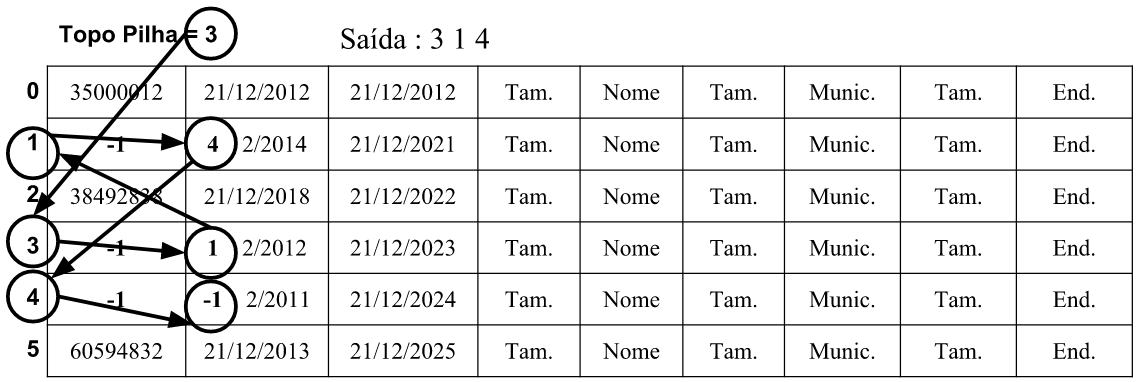
\includegraphics[width=\textwidth]{func9.png}
    \label{fig:func9}
\end{figure}

\end{document}